\documentclass[12pt]{article}
\usepackage[utf8]{inputenc}
\usepackage{amsmath}
\usepackage{graphicx}
\usepackage{booktabs}
\usepackage{hyperref}
\usepackage{float}
\usepackage{geometry}
\geometry{margin=1in}

\title{Homework 2 Report: Linear Regression\\
On the Auto Dataset}
\author {Thomas Meltesen}
\date{\today}

\begin{document}

\maketitle

\section{Introduction}
This report presents a linear regression with analysis on the Auto dataset to predict MPG using various vehicle features. For displacement, cylinders, weight, and acceleration as individual features.

\section{Methodology}

\subsection{Dataset}
The Auto dataset (\texttt{Auto.csv}) contains information about various automobile characteristics. For this assignment, we focus on predicting MPG (miles per gallon) using individual features.

\subsection{Data Preprocessing}
\begin{itemize}
    \item \textbf{Train-Test Split:} The dataset was randomly split into 60\% training data and 40\% test data.
    \item \textbf{Data Reshaping:} All features were reshaped from 1D pandas Series to 2D arrays to allow compatibility with the LinearRegression Model requirements.
\end{itemize}

\subsection{Model}
Using a simple linear regression models with the equation:
\begin{equation}
    \hat{y} = \beta_0 + \beta_1 x
\end{equation}
where $\hat{y}$ is the predicted MPG, $\beta_0$ is the intercept, $\beta_1$ is the slope (coefficient), and $x$ is the input feature.

\subsection{Evaluation Metrics}
Model performance was evaluated using:
\begin{itemize}
    \item \textbf{$R^2$ Score (Coefficient of Determination):} Measures the proportion of variance in MPG explained by the feature (range: 0 to 1)
    \item \textbf{MSE (Mean Squared Error):} Average squared difference between predicted and actual values.
\end{itemize}

\section{Results}

\subsection{Part A: Data Loading}
The Auto dataset was loaded using pandas. The displacement feature and MPG target variable were extracted.

\subsection{Part B: Data Splitting}
The dataset was split with the following:
\begin{itemize}
    \item Training set: 60\% of data
    \item Test set: 40\% of data
    \item Random state: 42 (for reproducibility)
\end{itemize}

\subsection{Part C: Initial Model - Displacement}
A linear regression model was trained using \textbf{displacement} as the predictor:

\begin{table}[H]
\centering
\begin{tabular}{lrrrrrr}
\toprule
\textbf{Parameter} & \textbf{Coef.} & \textbf{Std. Err.} & \textbf{t-stat} & \textbf{p-value} & $R^2$ & MSE \\
\midrule
Intercept ($\beta_0$) & 36.31 & 0.65 & 55.79 & $<0.001$ & 0.577 & 22.87 \\
Displacement ($\beta_1$) & -0.0639 & 0.0029 & -22.17 & $<0.001$ &  &  \\
\bottomrule
\end{tabular}
\caption{Linear regression parameters for Displacement vs MPG}
\end{table}

The negative slope indicates an inverse relationship: as displacement increases, MPG decreases which makes sense as the larger the displacement, the lower MPG, for larger vehicles.

\subsection{Part D: Model Evaluation - Displacement}
Performance metrics on the test set:

\begin{table}[H]
\centering
\begin{tabular}{lr}
\toprule
\textbf{Metric} & \textbf{Value} \\
\midrule
$R^2$ Score & 0.577 \\
MSE & 22.87 \\
\bottomrule
\end{tabular}
\caption{Performance metrics for Displacement model}
\end{table}

\subsection{Part E: Visualization - Displacement}
Figure \ref{fig:displacement} shows the test data scatter plot with the fitted regression line. The plot demonstrates a negative linear relationship with displacement and MPG. But the data would be better suited for a polynomial fit or other regression models to provide for a more suitable fit, as it has issues following the high variance around displacement of 50-150.

\begin{figure}[H]
    \centering
     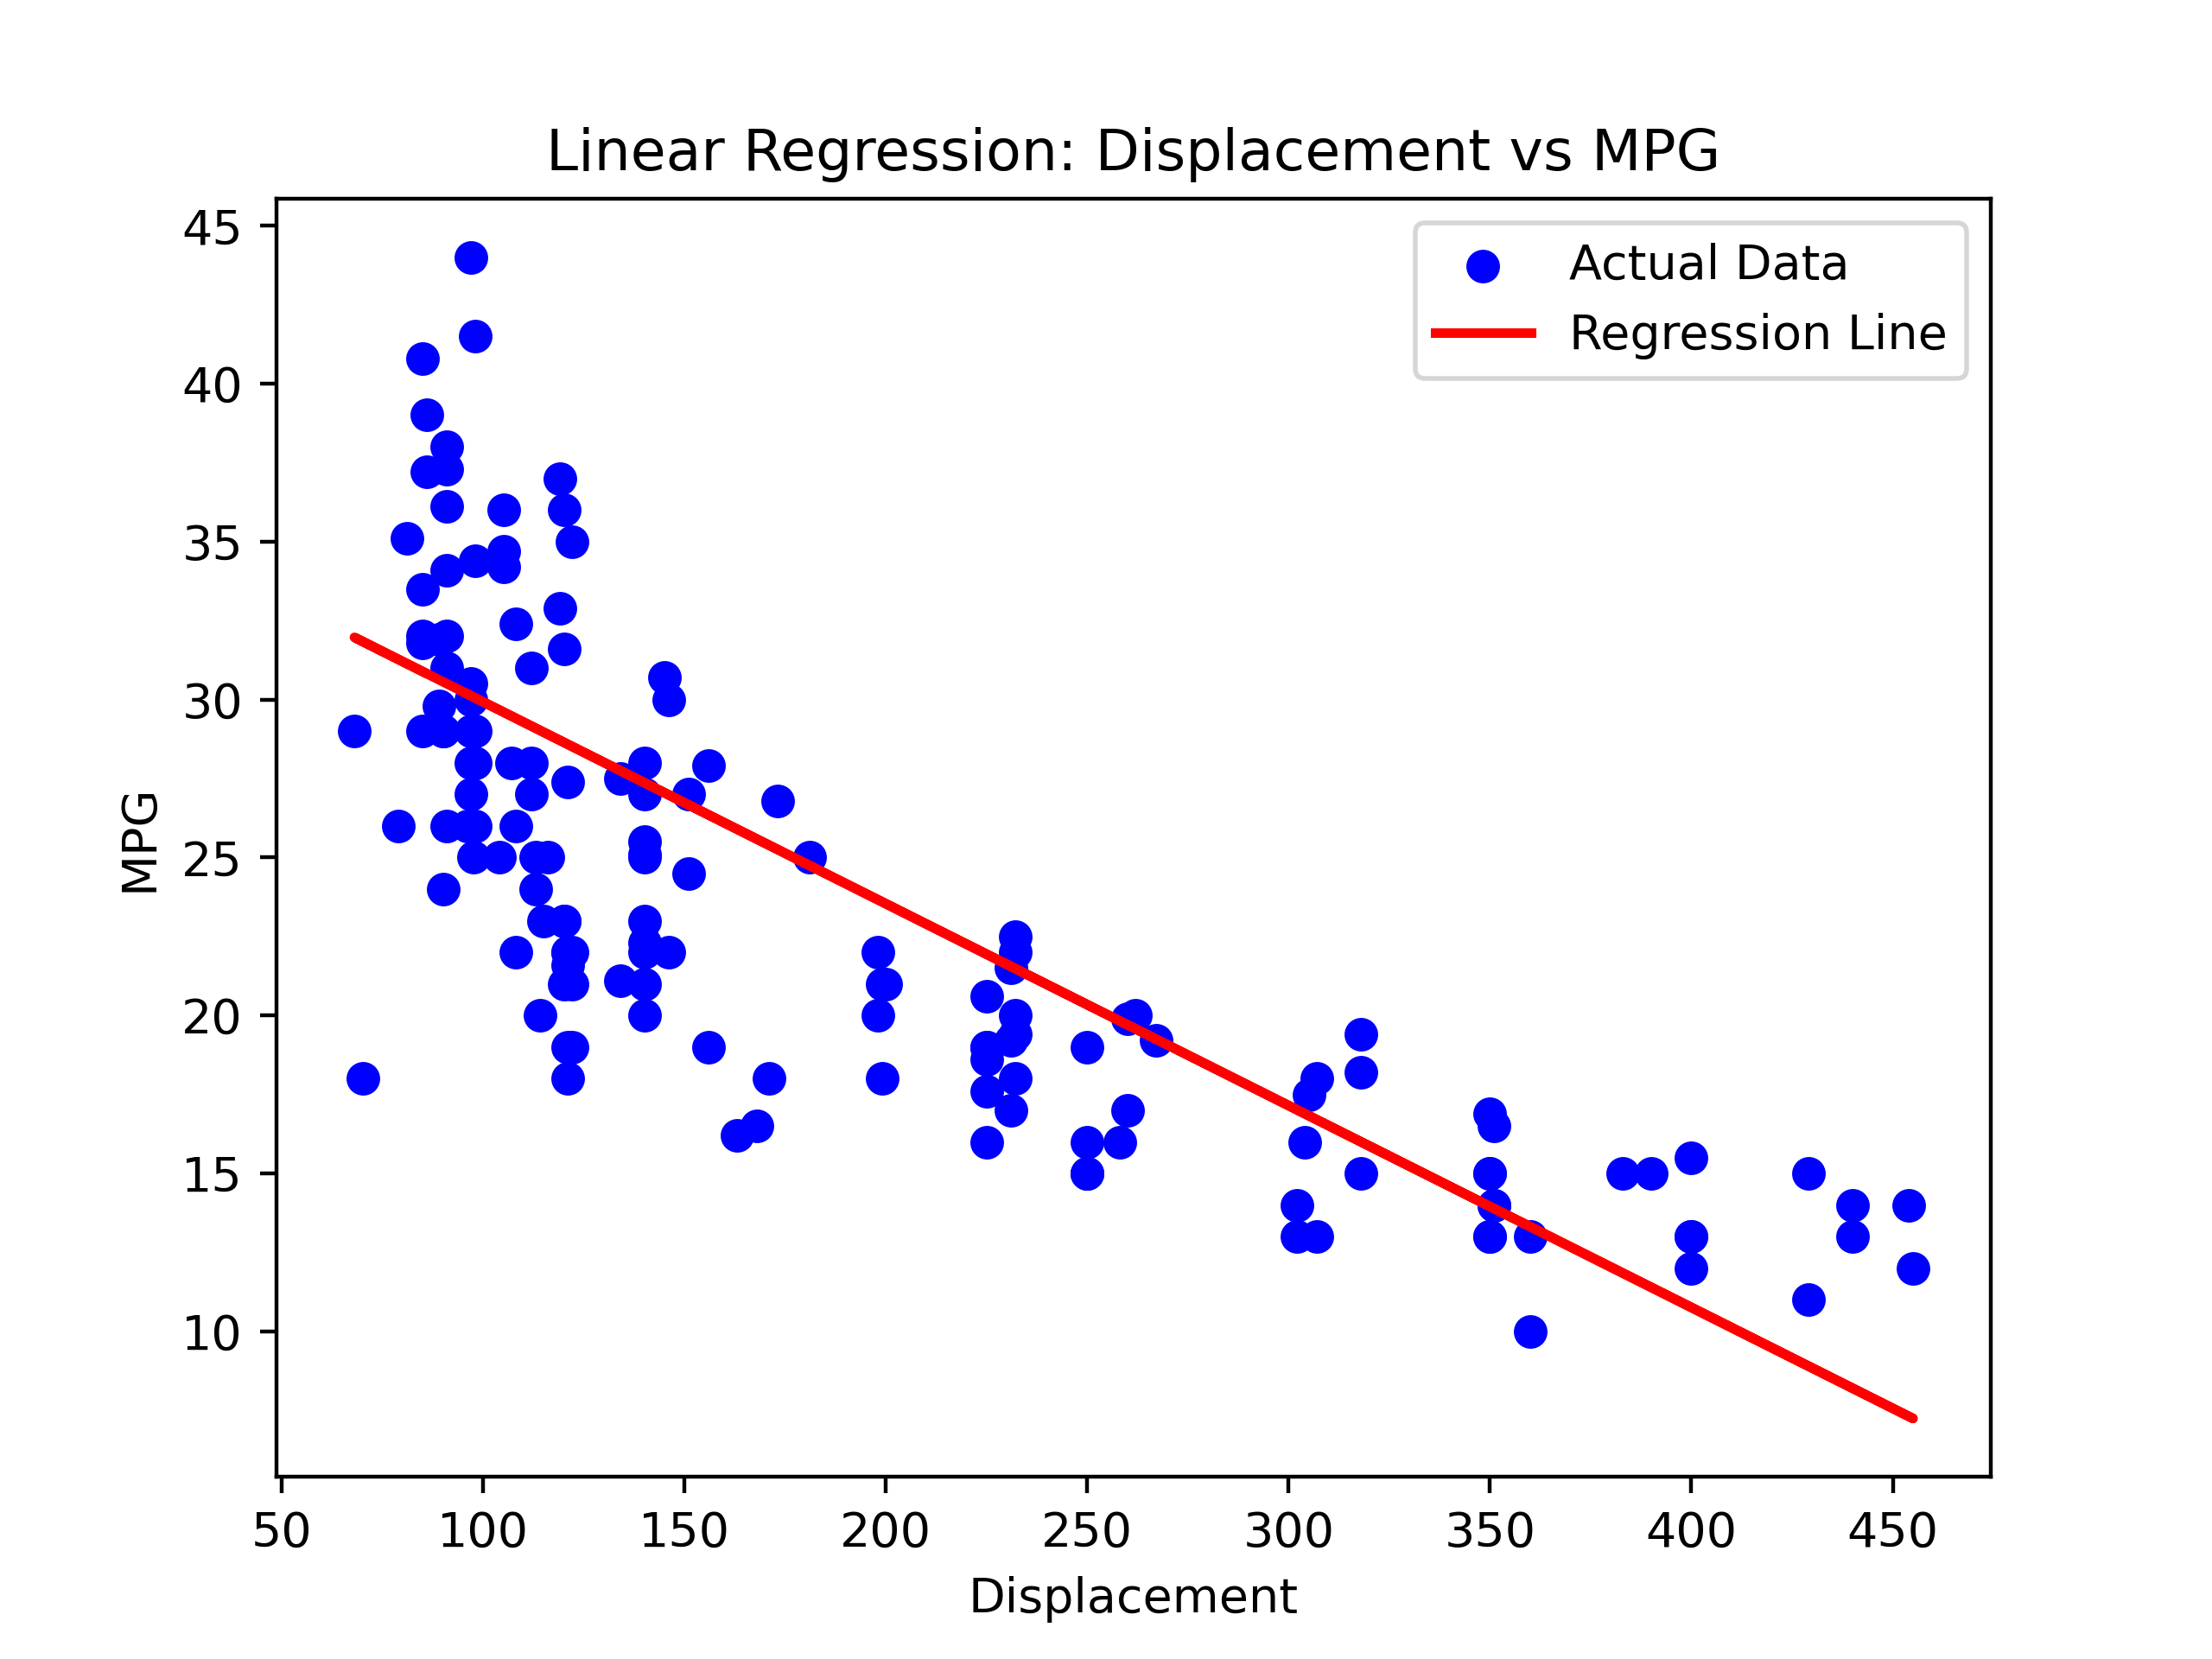
\includegraphics[width=0.7\textwidth]{Figure_Displacement.png}
    \caption{Linear regression: Displacement vs MPG with test data}
    \label{fig:displacement}
\end{figure}

\subsection{Part F: Additional Features}
Three additional features were used: cylinders, weight, and acceleration.

\subsubsection{Cylinders}
\begin{table}[H]
\centering
\begin{tabular}{lrrrrrr}
\toprule
\textbf{Parameter} & \textbf{Coef.} & \textbf{Std. Err.} & \textbf{t-stat} & \textbf{p-value} & $R^2$ & MSE \\
\midrule
Intercept ($\beta_0$) & 44.27 & 1.08 & 41.11 & $<0.001$ & 0.534 & 25.20 \\
Cylinders ($\beta_1$) & -3.7195 & 0.18 & -20.19 & $<0.001$ &  &  \\
\bottomrule
\end{tabular}
\caption{Model parameters and performance for Cylinders}
\end{table}

\subsubsection{Weight}
\begin{table}[H]
\centering
\begin{tabular}{lrrrrrr}
\toprule
\textbf{Parameter} & \textbf{Coef.} & \textbf{Std. Err.} & \textbf{t-stat} & \textbf{p-value} & $R^2$ & MSE \\
\midrule
Intercept ($\beta_0$) & 47.62 & 1.04 & 45.68 & $<0.001$ & 0.646 & 19.12 \\
Weight ($\beta_1$) & -0.0080 & 0.0003 & -24.04 & $<0.001$ &  &  \\
\bottomrule
\end{tabular}
\caption{Model parameters and performance for Weight}
\end{table}

\subsubsection{Acceleration}
\begin{table}[H]
\centering
\begin{tabular}{lrrrrrr}
\toprule
\textbf{Parameter} & \textbf{Coef.} & \textbf{Std. Err.} & \textbf{t-stat} & \textbf{p-value} & $R^2$ & MSE \\
\midrule
Intercept ($\beta_0$) & 3.60 & 2.60 & 1.39 & 0.167 & 0.124 & 47.35 \\
Acceleration ($\beta_1$) & 1.2907 & 0.166 & 7.79 & $<0.001$ &  &  \\
\bottomrule
\end{tabular}
\caption{Model parameters and performance for Acceleration}
\end{table}

\begin{figure}[H]
    \centering
     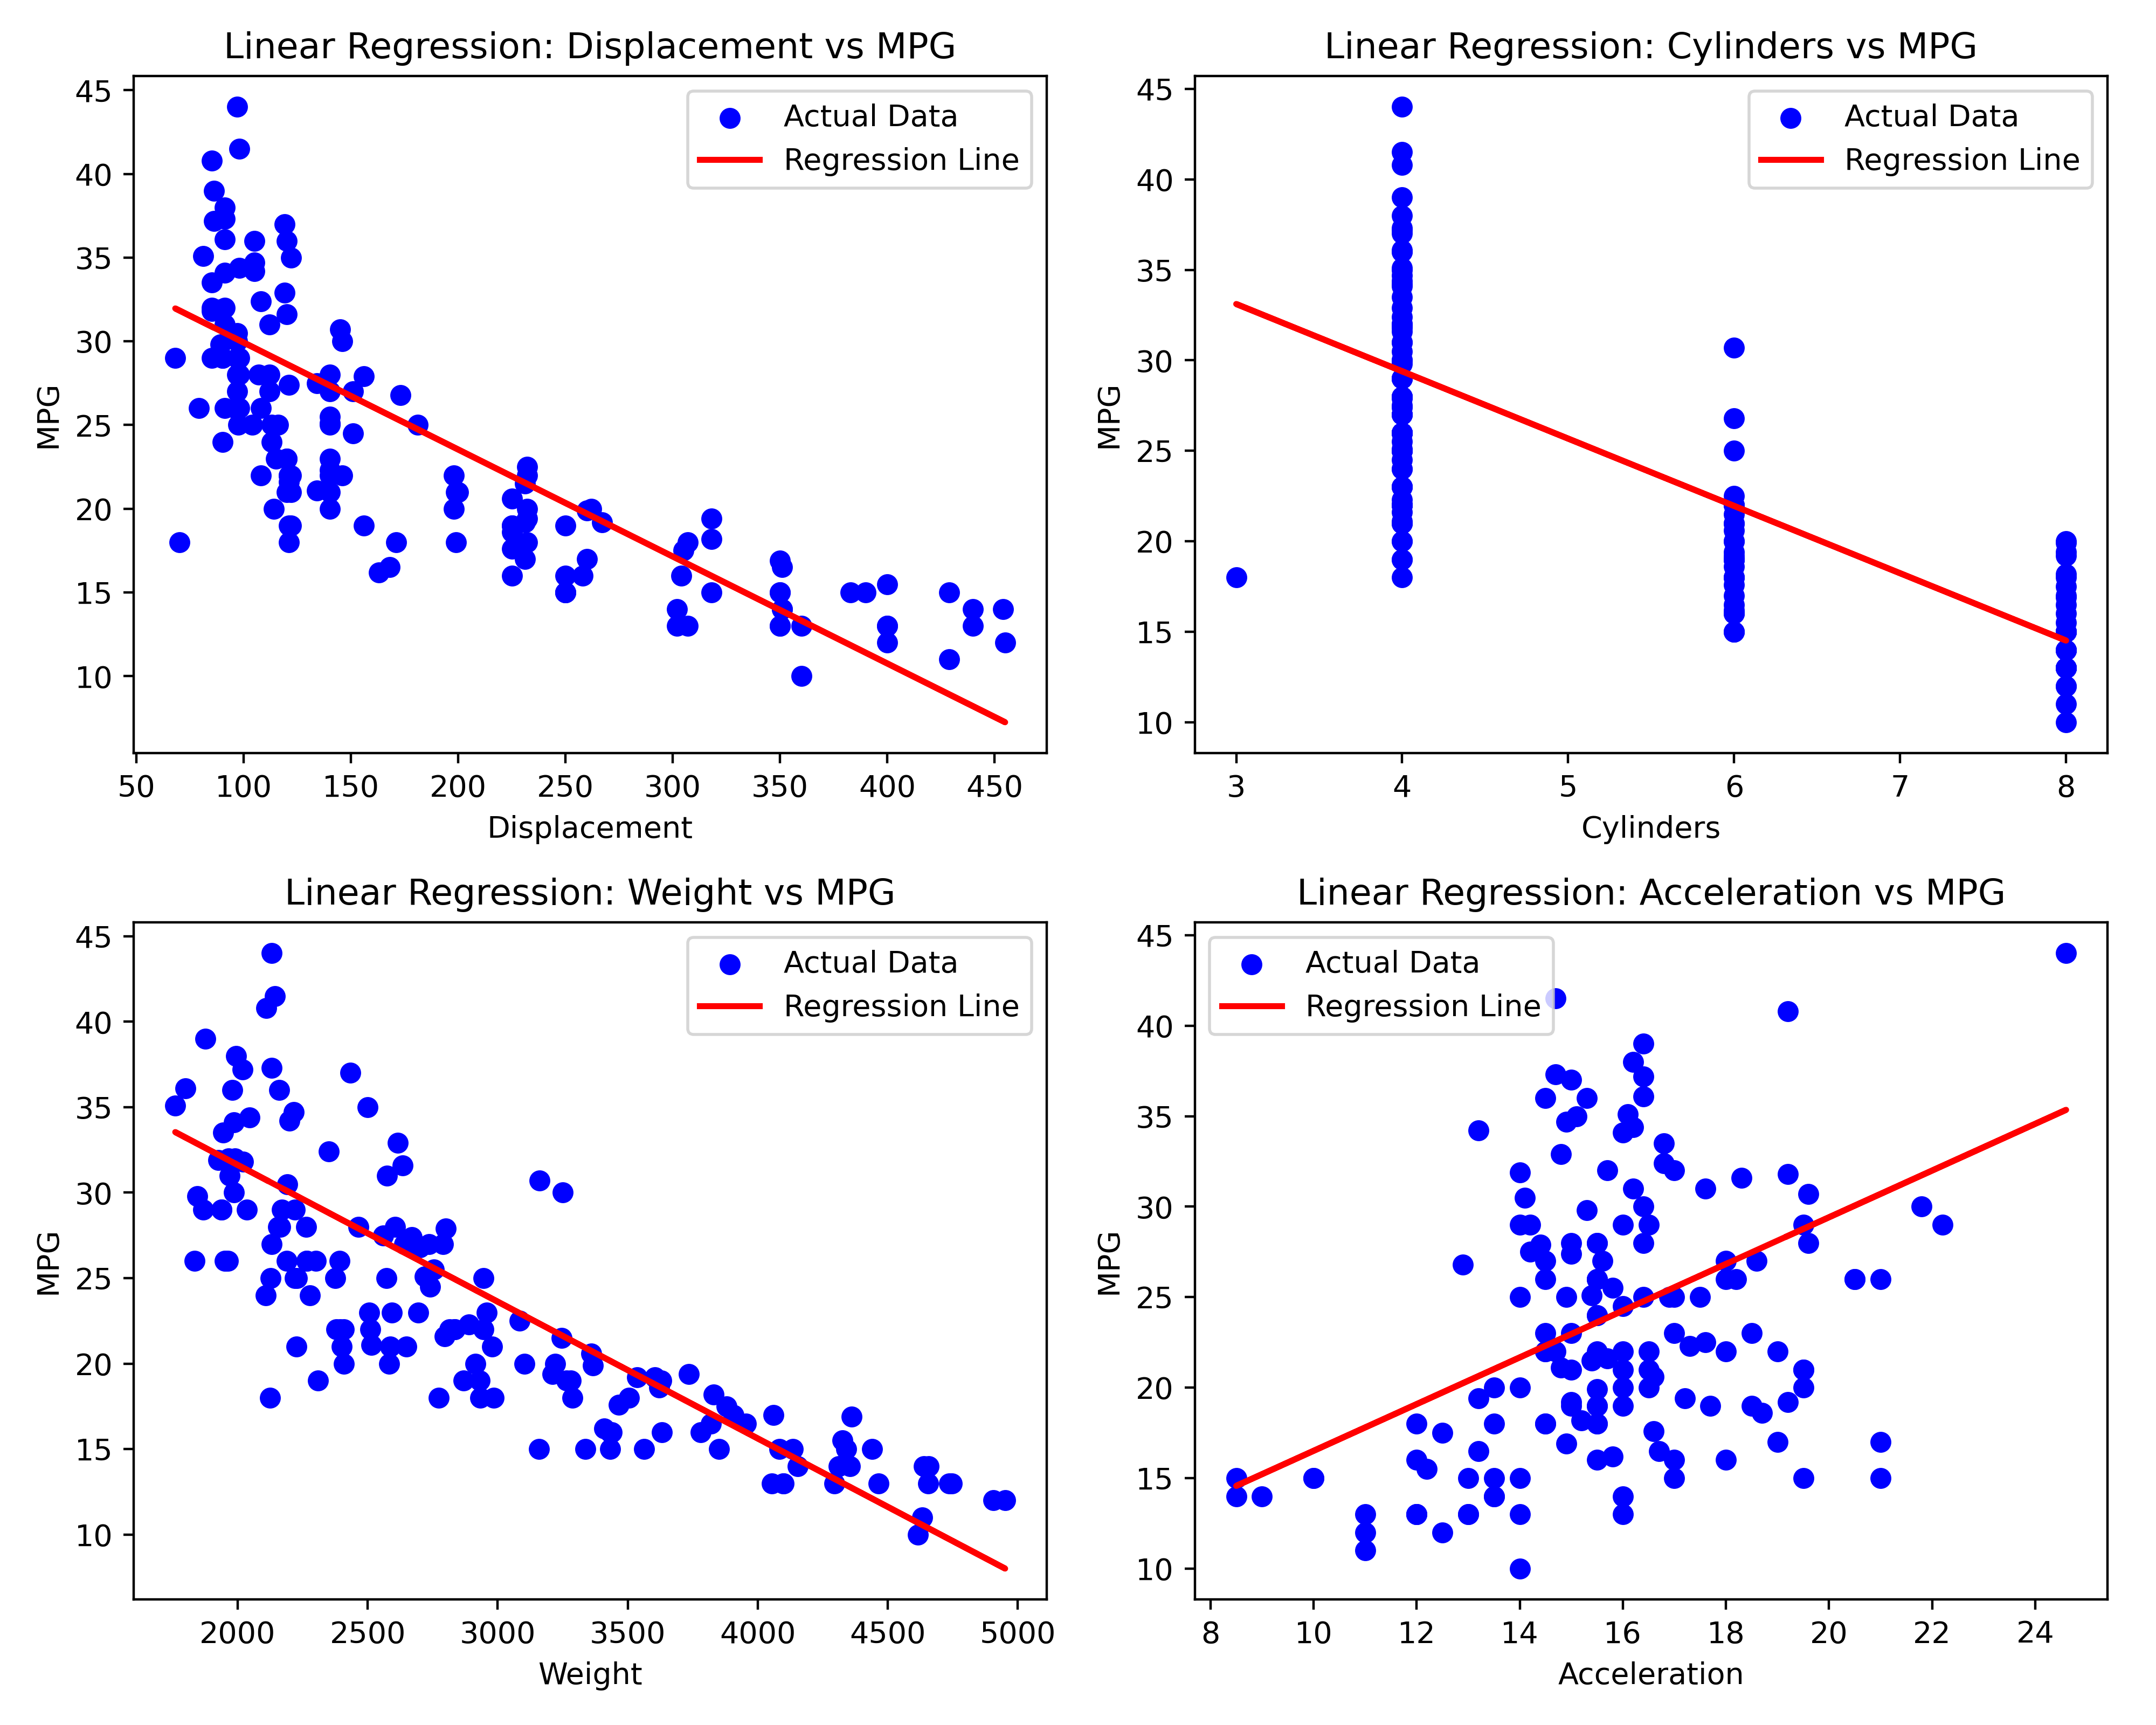
\includegraphics[width=\textwidth]{Figure_4Feats.png}
    \caption{Linear regression models for all four features (2×2 subplot grid)}
    \label{fig:all_features}
\end{figure}

\subsection{Part G: Feature Ranking}

\subsubsection{Ranking by MSE (Lower is Better)}
\begin{table}[H]
\centering
\begin{tabular}{clr}
\toprule
\textbf{Rank} & \textbf{Feature} & \textbf{MSE} \\
\midrule
1 & Weight & 19.12 \\
2 & Displacement & 22.87 \\
3 & Cylinders & 25.20 \\
4 & Acceleration & 47.35 \\
\bottomrule
\end{tabular}
\caption{Feature ranking by Mean Squared Error}
\label{tab:mse_ranking}
\end{table}

\subsubsection{Ranking by $R^2$ Score (Higher is Better)}
\begin{table}[H]
\centering
\begin{tabular}{clr}
\toprule
\textbf{Rank} & \textbf{Feature} & \textbf{$R^2$ Score} \\
\midrule
1 & Weight & 0.646 \\
2 & Displacement & 0.577 \\
3 & Cylinders & 0.534 \\
4 & Acceleration & 0.124 \\
\bottomrule
\end{tabular}
\caption{Feature ranking by $R^2$ Score}
\label{tab:r2_ranking}
\end{table}

\section{Discussion}

\subsection{Key Findings}
\begin{itemize}
    \item \textbf{Best Predictor:} Weight demonstrated the strongest predictive power for MPG, with a highly significant coefficient ($p<0.001$, $t=-24.04$), the highest $R^2$ score (0.646), and lowest MSE (19.12).
    \item \textbf{Weakest Predictor:} Acceleration showed the poorest performance with a significant coefficient ($p<0.001$, $t=7.79$), but a low $R^2$ (0.124) and high MSE (47.35). The intercept for acceleration was not statistically significant ($p=0.167$).
    \item \textbf{Physical Interpretation:} The negative slopes for displacement, cylinders, and weight indicate that larger, heavier vehicles with more cylinders tend to have lower fuel efficiency.
\end{itemize}

\subsection{Model Performance}
All features show weak to moderate linear relationships with MPG. The $R^2$ values range from 0.124 to 0.646. For all features except the intercept in the acceleration model, the coefficients are highly statistically significant ($p<0.001$), supporting a real relationship, but only weight provides strong predictive power. Simple linear models only capture part of the variance.

\subsection{Limitations}
\begin{itemize}
    \item Simple linear regression captures only linear relationships; non-linear patterns may exist.
    \item Single-feature models ignore interactions between variables (e.g., weight and displacement are likely correlated).
    \item Model assumes homoscedasticity and normally distributed residuals (not verified in this analysis).
\end{itemize}
\begin{figure}
    \centering
    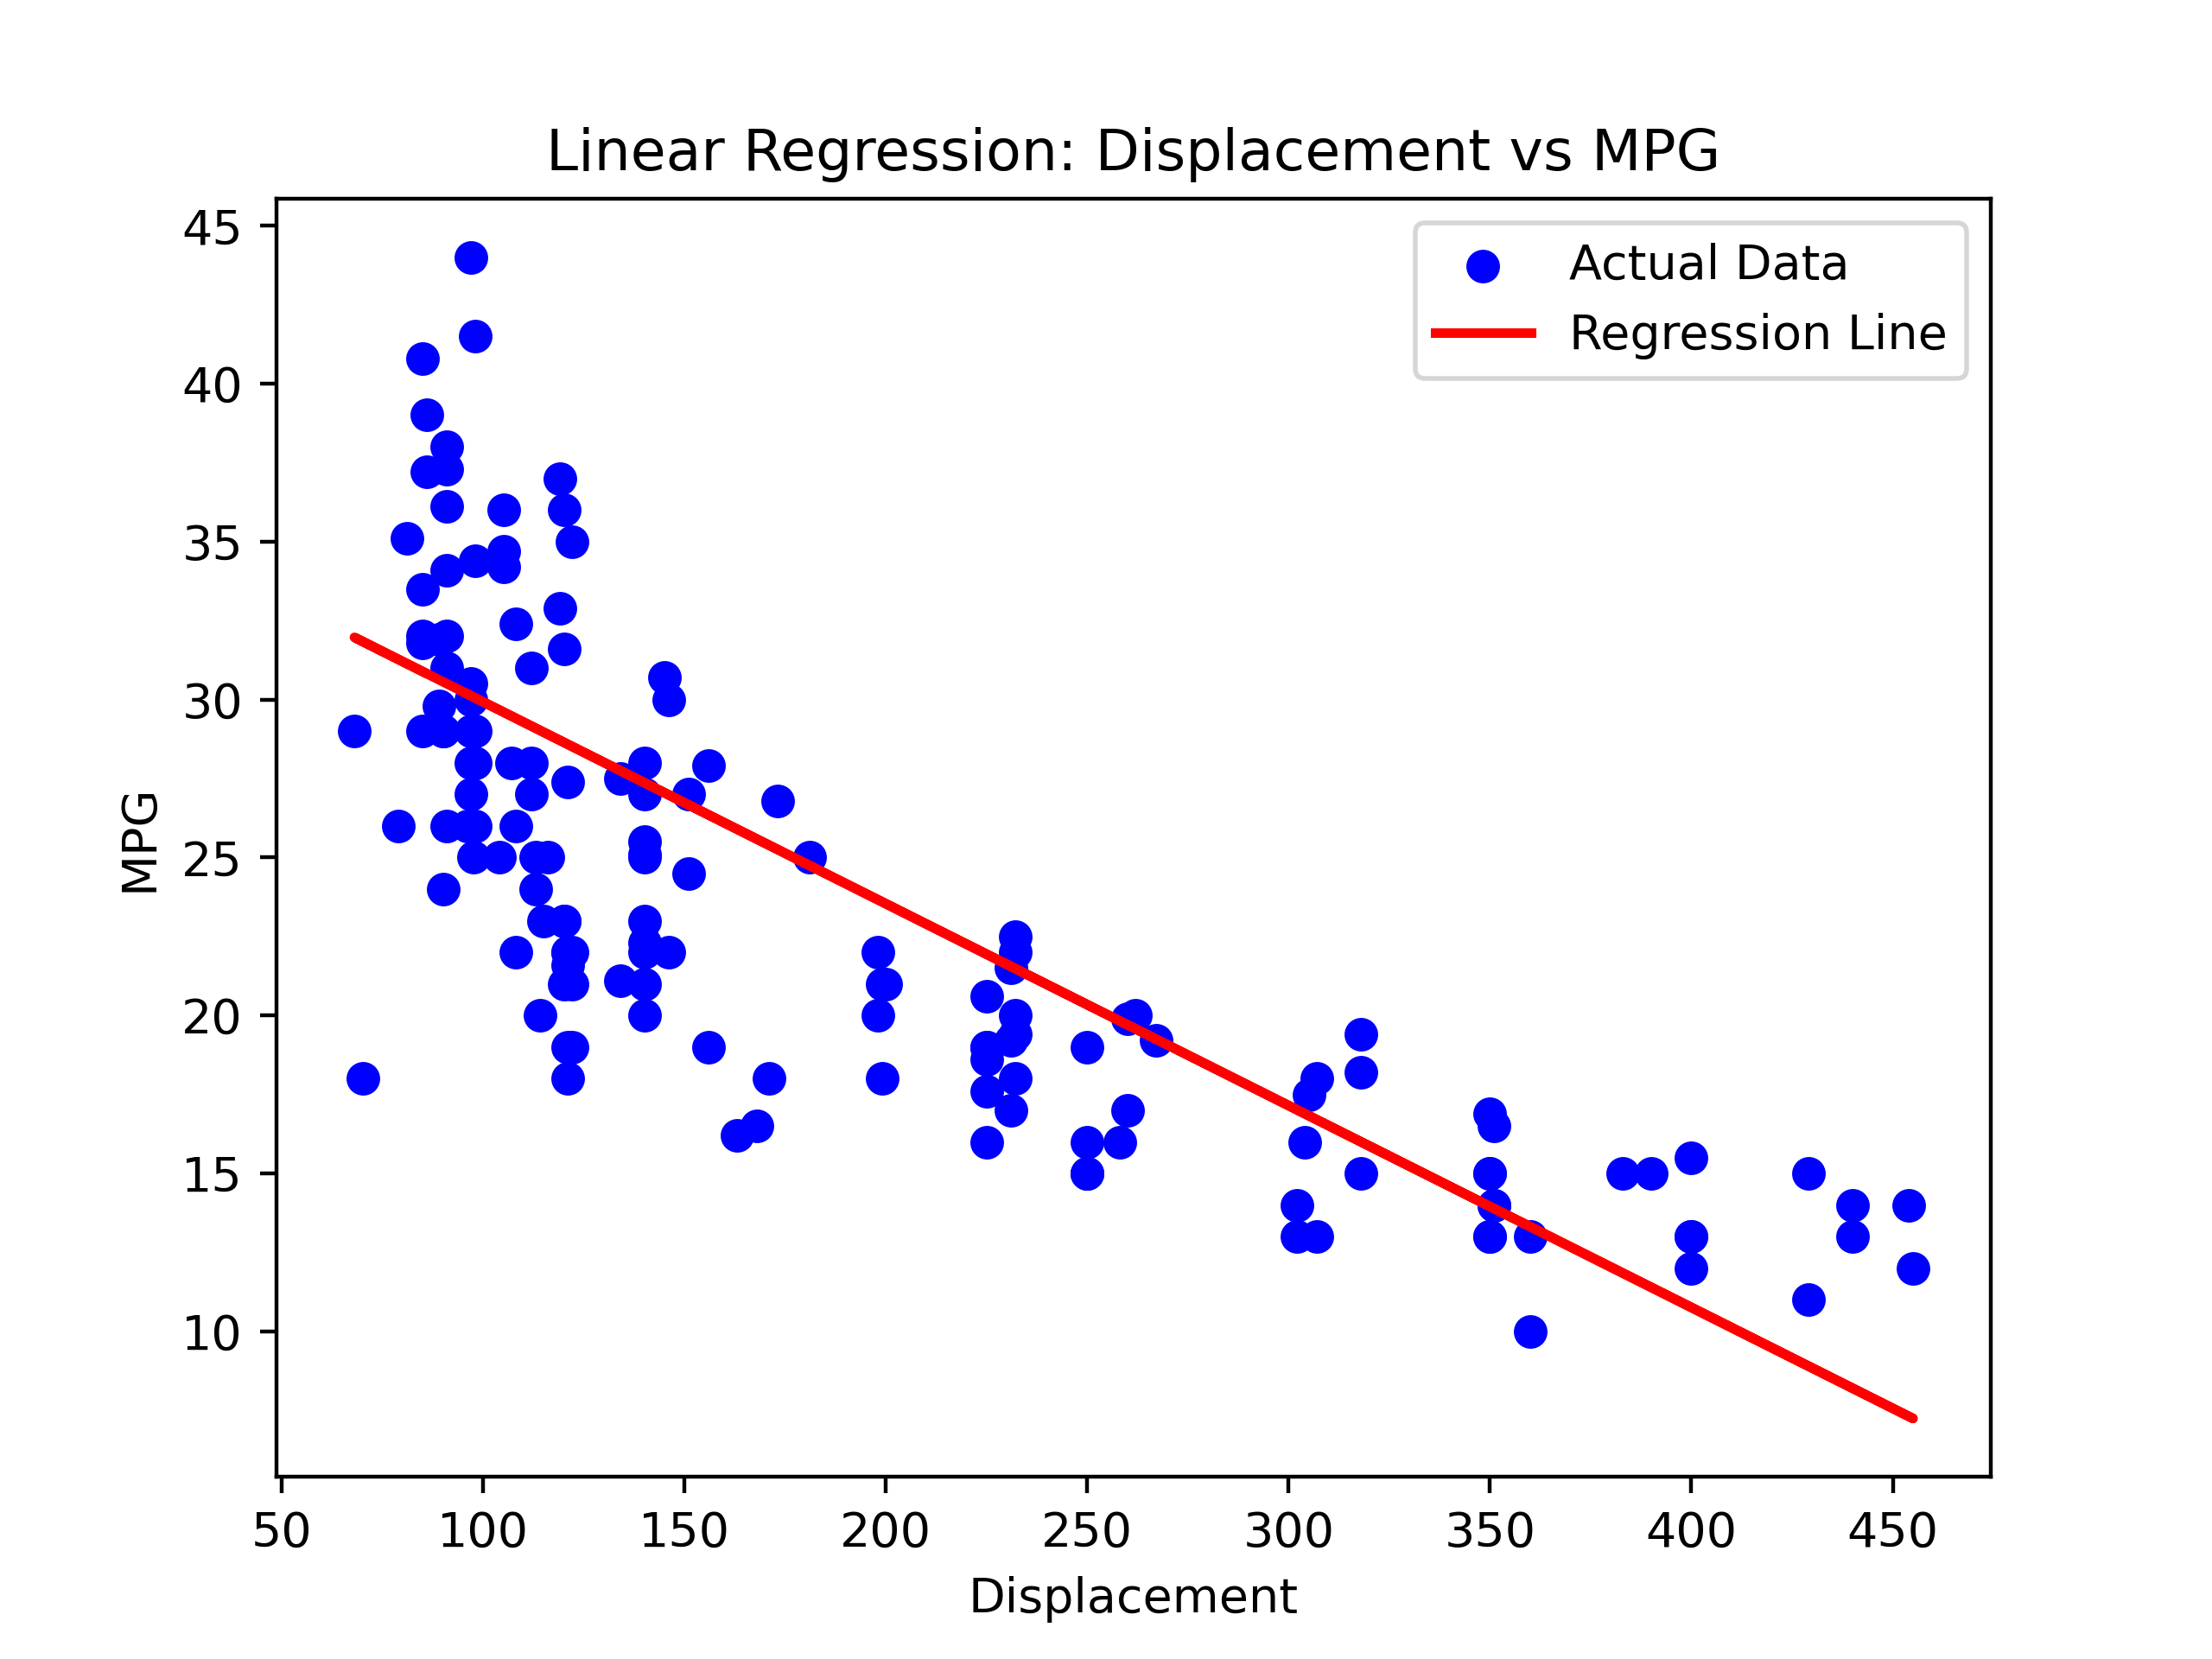
\includegraphics[width=0.5\linewidth]{Figure_Displacement.png}
    \caption{Enter Caption}
    \label{fig:placeholder}
\end{figure}

\section{Conclusion}
This analysis successfully demonstrated the application of simple linear regression to predict automobile fuel efficiency. Among the four features analyzed (displacement, cylinders, weight, acceleration), weight emerged as the strongest predictor of MPG. The results provide valuable insights into the factors affecting fuel economy and establish a foundation for more sophisticated multi-feature models.

\section{Disclaimers}
\begin{itemize}
    \item All Python code for data processing, model training, and visualization is available in the Jupyter notebook (\texttt{hw2.ipynb}).
    
    \item This LaTex document was formatted and generated by AI. All data, images and text were written in spaces by me to provide for a properly formatted report and ensure readability.

    \item Additionally, I used AI assistance in the code part as a tool to help and learn how to plot the models and enumerate through the different model performance metrics.
\end{itemize}
\end{document}
